\documentclass[a4paper,11pt]{article}
\usepackage[margin=1in]{geometry}
\usepackage{tikz,tkz-graph,graphicx}
\usepackage{xcolor}
\usepackage{subcaption}

\usetikzlibrary{arrows.meta,positioning,shapes,chains,calc,math}

\definecolor{lightOrange}{rgb}{0.9921875,0.890625,0.69921875}
\definecolor{darkOrange}{rgb}{0.96875,0.64453125,0.33203125}
\definecolor{skyBlue}{rgb}{0.66796875,0.875,0.97265625}
\definecolor{darkBlue}{rgb}{0.046875,0.69140625,0.9375}

\begin{document}

\section*{Picture}
\begin{figure}[h]
	\centering
	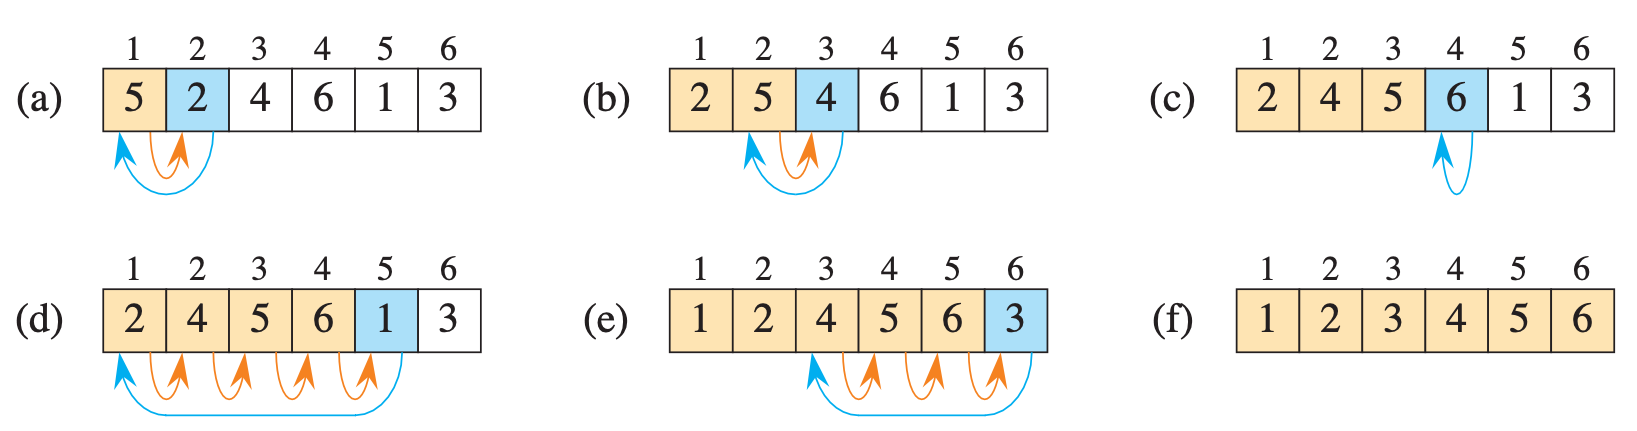
\includegraphics[width=0.7\textwidth]{./5.png}
\end{figure}

\section*{PDF}
\begin{figure}[h]
  \begin{subfigure}[T]{0.3\textwidth}\vskip 0pt
    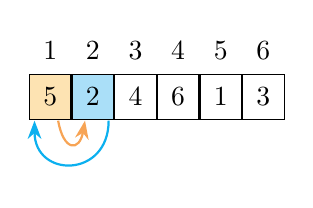
\begin{tikzpicture}[
      >=Stealth,
      every node/.style={
        inner sep=5pt,
        anchor=south,
        draw
      },
      node distance=0pt,
      start chain
      ]
      
      \node[on chain,label=above:1, fill=lightOrange] (1) {5};
      \node[on chain,label=above:2, fill=skyBlue] (2) {2};

      \foreach \i/\j in {3/4, 4/6, 5/1, 6/3}{
        \node[on chain, label=above:\i] (\i) {\j};
      }
      
      \draw[->, looseness=2, thick, color=darkBlue]
      ($(2)+(0.2,-0.3)$) to[out=270, in=270] ($(1)+(-0.2,-0.3)$);
      
      \draw[->, looseness=3, thick, color=darkOrange]
      ($(1)+(0.1,-0.3)$) to[out=280,in=260] ($(2)+(-0.1,-0.3)$);
    \end{tikzpicture}
    \caption{~}
  \end{subfigure}\hfill\begin{subfigure}[T]{0.3\textwidth}\vskip 0pt
    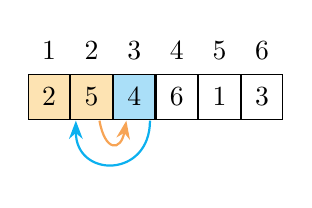
\begin{tikzpicture}[
      >=Stealth,
      every node/.style={
      inner sep=5pt,
      anchor=south,
      draw
    },
      node distance=0pt,
      start chain
      ]

      \node[on chain,label=above:1, fill=lightOrange] (1) {2};
      \node[on chain,label=above:2, fill=lightOrange] (2) {5};
      \node[on chain,label=above:3, fill=skyBlue] (3) {4};

      \foreach \i/\j in {4/6, 5/1, 6/3}{
        \node[on chain, label=above:\i] (\i) {\j};
      }
      
      \draw[->, looseness=2, thick, color=darkBlue]
      ($(3)+(0.2,-0.3)$) to[out=270, in=270] ($(2)+(-0.2,-0.3)$);
    
      \draw[->, looseness=3, thick, color=darkOrange]
      ($(2)+(0.1,-0.3)$) to[out=280,in=260] ($(3)+(-0.1,-0.3)$);
    \end{tikzpicture}
    \caption{~}
  \end{subfigure}\hfill\begin{subfigure}[T]{0.3\textwidth}\vskip 0pt
    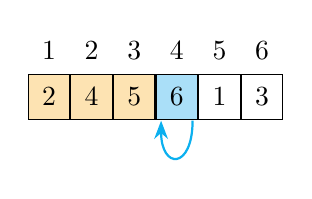
\begin{tikzpicture}[
      >=Stealth,
      every node/.style={
        inner sep=5pt,
        anchor=south,
        draw
      },
      node distance=0pt,
      start chain
      ]

      \foreach \i/\j in {1/2, 2/4, 3/5}{
        \node[on chain,label=above:\i, fill=lightOrange] (\i) {\j};
      }

      \node[on chain,label=above:4, fill=skyBlue] (4) {6};
      \node[on chain,label=above:5] (5) {1};
      \node[on chain,label=above:6] (6) {3};
      
      \draw[->, looseness=4, color=darkBlue, thick]
      ($(4)+(0.2,-0.3)$) to[out=270, in=270] ($(4)+(-0.2,-0.3)$);
    \end{tikzpicture}
    \caption{~}
  \end{subfigure}

  \begin{subfigure}[T]{0.3\textwidth}\vskip 0pt
    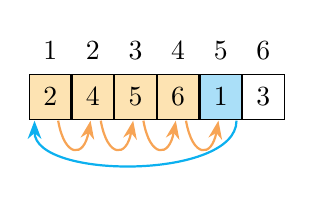
\begin{tikzpicture}[
      >=Stealth,
      every node/.style={
        inner sep=5pt,
        anchor=south,
        draw
      },
      node distance=0pt,
      start chain
      ]

      \foreach \i/\j in {1/2, 2/4, 3/5, 4/6}{
        \node[on chain,label=above:\i, fill=lightOrange] (\i) {\j};
      }
     \node[on chain,label=above:5, fill=skyBlue] (5) {1};
      \node[on chain,label=above:6] (6) {3};
      
      \foreach \i in {1,...,4}{
        \tikzmath{
          \j=\i+1;
        }
        \draw[->, looseness=3, thick, color=darkOrange]
        ($(\i)+(0.1,-0.3)$) to[out=280,in=260] ($(\j)+(-0.3,-0.3)$);
      }
      
      \draw[->, looseness=0.75, color=darkBlue, thick]
      ($(5)+(0.2,-0.3)$) to[out=270, in=270] ($(1)+(-0.2,-0.3)$);
    \end{tikzpicture}
    \caption{~}
  \end{subfigure}\hfill\begin{subfigure}[T]{0.3\textwidth}\vskip 0pt
    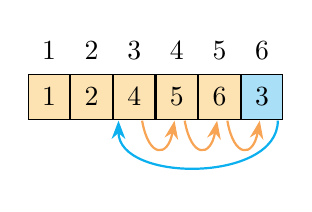
\begin{tikzpicture}[
      >=Stealth,
      every node/.style={
        inner sep=5pt,
        anchor=south,
        draw
      },
      node distance=0pt,
      start chain
      ]

      \foreach \i/\j in {1/1, 2/2, 3/4, 4/5, 5/6}{
        \node[on chain,label=above:\i, fill=lightOrange] (\i) {\j};
      }
      \node[on chain,label=above:6, fill=skyBlue] (6) {3};
      
      \foreach \i in {3,...,5}{
        \tikzmath{
          \j=\i+1;
        }
        \draw[->, looseness=3, thick, color=darkOrange]
        ($(\i)+(0.1,-0.3)$) to[out=280,in=260] ($(\j)+(-0.3,-0.3)$);
      }
      \draw[->, looseness=1, color=darkBlue, thick]
      ($(6)+(0.2,-0.3)$) to[out=270, in=270] ($(3)+(-0.2,-0.3)$);
    \end{tikzpicture}
    \caption{~}
  \end{subfigure}\hfill\begin{subfigure}[T]{0.3\textwidth}\vskip 0pt
    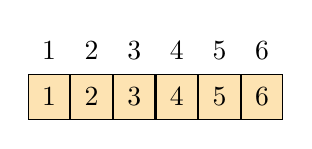
\begin{tikzpicture}[
      >=Stealth,
      every node/.style={
        inner sep=5pt,
        anchor=south,
        draw
      },
      node distance=0pt,
      start chain
      ]
      
      \foreach \i in {1,...,6}{
        \node[on chain,label=above:\i, fill=lightOrange] (\i) {\i};
      }
    \end{tikzpicture}
    \caption{~}
  \end{subfigure}
\end{figure}
\end{document}